%=====================================================================
% TÀI LIỆU BỔ TRỢ — bản nguồn, không được \input{} vào thân bài chính
% Mục đích: giữ chi tiết tái lập/traceability bên ngoài bài báo khoa học.
%=====================================================================
\documentclass[a4paper,11pt]{article}
\usepackage{fontspec}
\IfFontExistsTF{Times New Roman}{\setmainfont{Times New Roman}}{\setmainfont{DejaVu Serif}}
\usepackage[a4paper,top=2cm,bottom=2cm,left=2.2cm,right=2.2cm]{geometry}
\usepackage{booktabs,tabularx,longtable,array}
\usepackage{graphicx}
\usepackage{amsmath}
\usepackage{hyperref}
\usepackage{enumitem}
\setlist{nosep,leftmargin=*}
\setlength{\parindent}{1.2cm}
\setlength{\parskip}{3pt}

\begin{document}
\begin{center}
{\bfseries TÀI LIỆU BỔ TRỢ\\
Kiến trúc tham chiếu tỉnh--trung ương cho nền tảng số quản lý DN KH\&CN và DN KNST}
\end{center}

\section*{S1. Tập nguồn và nguyên tắc lựa chọn}
Tập nguồn được khóa theo trạng thái đến 08/08/2026. Việc lựa chọn tài liệu tuân theo bốn quy tắc:
\begin{enumerate}[label=\textbf{D\arabic*.}]
\item Khởi tạo từ các văn bản hiện hành trực tiếp điều chỉnh DN KH\&CN/DN KNST và các khung kiến trúc, dữ liệu, định danh, liên thông, bảo vệ dữ liệu có tác động tới nền tảng.
\item Lần theo văn bản sửa đổi, thay thế hoặc được dẫn chiếu khi chúng làm thay đổi một nghĩa vụ có hệ quả kiến trúc.
\item Chỉ đưa vào tập ràng buộc tài liệu có mệnh đề tác động trực tiếp tới dữ liệu, quy trình, thẩm quyền, vòng đời, kết nối/chia sẻ, bảo vệ, báo cáo hoặc kiểm soát. Tài liệu học thuật chỉ dùng cho nền tảng lý thuyết và không sinh ràng buộc chuẩn tắc.
\item Khóa trạng thái tại ngày cắt; tách dự thảo và nguồn phương pháp khỏi nguồn tạo nghĩa vụ.
\end{enumerate}

Nguồn được chia thành ba lớp: \textbf{A}--hiện hành/có thẩm quyền, tạo đường cơ sở; \textbf{D}--dự thảo, chỉ dùng chẩn đoán; \textbf{M}--phương pháp/tham chiếu quốc tế. Danh mục cấp tài liệu, trạng thái, đường đưa vào và lý do lựa chọn nằm trong \texttt{corpus\_manifest.csv}. Cách phân lớp này nhằm ngăn dự thảo hoặc nguồn tham chiếu quốc tế bị diễn giải như nghĩa vụ pháp lý Việt Nam.

\section*{S2. Quy tắc nguyên tử hóa ràng buộc}
C01--C10 là các họ ràng buộc; đơn vị truy vết Cxx.yy là một mệnh đề ràng buộc nguồn có vị trí dẫn chiếu cụ thể. Từ 116 đơn vị nguồn, quy trình tạo 128 dòng truy vết, gồm 114 lớp A, 8 lớp D và 6 lớp M.

\begin{table}[ht]
\centering
\small
\begin{tabularx}{\textwidth}{>{\bfseries}p{0.7cm}X}
\toprule
R1 & Chọn đơn vị nguồn nhỏ nhất có vị trí dẫn chiếu đủ chính xác và có nội dung liên quan trực tiếp tới kiến trúc; một đơn vị chỉ sinh một Cxx.yy nếu có một tiêu chí kiểm tra độc lập.\\
R2 & Tách một đơn vị nguồn thành nhiều Cxx.yy khi các nghĩa vụ, quyền, trạng thái hoặc thời hạn có thể được kiểm tra độc lập.\\
R3 & Giữ riêng các mệnh đề tương đồng nằm ở nguồn hoặc vị trí dẫn chiếu khác nhau để bảo toàn xuất xứ; nhiều mệnh đề có thể cùng ánh xạ tới một quyết định hoặc thành phần kiến trúc.\\
R4 & Chỉ mệnh đề minh thị từ nguồn lớp A mới được gán L1. D và M không tạo L1; L2/L3 là đáp ứng hoặc suy luận thiết kế và không được tính thêm vào 128 dòng nguồn.\\
R5 & Mỗi Cxx.yy phải có nguồn--vị trí dẫn chiếu, loại/mức căn cứ, đáp ứng kiến trúc, thành phần liên quan, tiêu chí kiểm tra và trạng thái. Trạng thái phản ánh mức đáp ứng ở thời điểm thiết kế, không phải chứng nhận tuân thủ của hệ thống đã triển khai.\\
\bottomrule
\end{tabularx}
\end{table}

\section*{S3. Ví dụ mã hóa và truy vết}
\textbf{Ví dụ một--nhiều.} Một đơn vị nguồn chứa nhiều nghĩa vụ có tiêu chí kiểm tra khác nhau được tách thành nhiều Cxx.yy. Trường hợp điểm c khoản 2 Điều 43 NĐ 268 được tách thành C03.18--C03.22 tương ứng với khả năng lập Hội đồng và các mốc thời hạn khác nhau. Mục tiêu của phép tách là cho phép kiểm tra từng nghĩa vụ thay vì gán một trạng thái chung cho cả đoạn luật.

\textbf{Ví dụ truy vết.} Khoản 2 Điều 66 NĐ 268 tạo C03.46 về nghĩa vụ cấp tỉnh thông báo Bộ trong thời hạn quy định. C03.46 được nối tới quyết định kiến trúc và các thành phần chịu trách nhiệm về trạng thái, thời hạn, thông báo và điều phối. Nghĩa vụ thời hạn là L1; dấu thời gian, theo dõi hạn, xác nhận nhận và gửi lại có kiểm soát là L2; công nghệ hàng đợi hoặc middleware cụ thể là L3. Tiêu chí kiểm tra đặt hệ thống vào tình huống lớp trung ương tạm không sẵn sàng để xem nghĩa vụ thông báo có được bảo toàn mà không làm mất trạng thái nghiệp vụ hay không.

Các ví dụ chi tiết khác và toàn bộ locator nguồn nằm trong \texttt{source\_unit\_index.csv} và \texttt{constraint\_traceability.csv}.

\section*{S4. Chuỗi truy vết kiến trúc}
Chuỗi truy vết chuẩn là:
\[
\text{nguồn/vị trí}\rightarrow \text{Cxx.yy}\rightarrow \text{DRV/AD/AE}\rightarrow \text{tiêu chí kiểm tra}\rightarrow \text{trạng thái}.
\]
Chiều thuận dùng để giải thích căn cứ của quyết định kiến trúc; chiều ngược dùng để phát hiện thành phần không có căn cứ nguồn hoặc chỉ là lựa chọn thiết kế. Các bảng máy đọc được tương ứng được lưu riêng theo nhóm động lực, quyết định, thành phần, điểm biến thiên và quy tắc phù hợp.

Ba mức căn cứ được sử dụng xuyên suốt:
\begin{itemize}
\item \textbf{L1}: nghĩa vụ/cấu trúc/mốc thời gian được nguồn lớp A quy định minh thị;
\item \textbf{L2}: hệ quả kiến trúc suy ra trực tiếp để đáp ứng L1;
\item \textbf{L3}: lựa chọn hiện thực hóa cần được kiểm chứng khi triển khai.
\end{itemize}

\section*{S5. Giao thức lựa chọn và chấm kịch bản}
Mười kịch bản S1--S10 được xây dựng để phủ năm nhóm mối quan tâm:
\begin{enumerate}
\item vận hành bình thường và biến thể địa phương (S1--S2);
\item thay đổi quy định, nguồn hoặc phiên bản (S3, S6, S10);
\item gián đoạn hạ tầng/lớp trung ương (S4, S7);
\item tổng hợp toàn quốc và quan hệ xuyên địa bàn (S5, S8);
\item chuyển giao phạm vi quản lý/ghi giữa địa bàn (S9).
\end{enumerate}
Ma trận \texttt{scenario\_coverage.csv} kiểm tra mỗi động lực kiến trúc xuất hiện trong ít nhất hai kịch bản và mỗi góc nhìn được thử thách bởi ít nhất một kịch bản. Tiêu chí này chỉ mô tả độ phủ, không tạo trọng số hoặc điểm tổng hợp.

Rubric ba mức:
\begin{itemize}
\item \textsc{Đáp ứng trực tiếp}: lõi kiến trúc xử lý kịch bản mà không cần sửa quyết định ổn định;
\item \textsc{Đáp ứng có điều kiện}: cần cụ thể hóa hoặc kiểm chứng một cơ chế/điểm biến thiên đã được kiến trúc cho phép;
\item \textsc{Rủi ro kiến trúc}: kịch bản buộc phải xem xét lại một quyết định/lõi ổn định hoặc còn điểm thẩm quyền, toàn vẹn hay tương thích chưa giải quyết.
\end{itemize}

B1$_0$ được chấm trước tinh chỉnh. Khi S9 và S10 làm lộ khoảng trống, các thay đổi được ghi vào nhật ký tinh chỉnh và tạo B1-R; sau đó cùng bộ S1--S10 và cùng rubric được áp dụng lại. Kết quả chi tiết nằm trong \texttt{evaluation\_results.csv}, \texttt{evaluation\_results\_b1r.csv} và \texttt{architecture\_refinement\_log.csv}.

\section*{S6. Phạm vi tái lập và phiên bản chứng cứ}
Các tệp bổ trợ chính gồm:
\begin{itemize}
\item \texttt{corpus\_manifest.csv}, \texttt{source\_unit\_index.csv};
\item \texttt{constraint\_traceability.csv};
\item các sổ DRV/AD/AE/VP/CR;
\item \texttt{evaluation\_scenarios.csv}, \texttt{evaluation\_rubric.csv}, \texttt{scenario\_coverage.csv};
\item kết quả B1$_0$/B1-R và nhật ký tinh chỉnh;
\item các tệp nguồn sinh hình trong thư mục \texttt{figure\_sources/}.
\end{itemize}

Trước khi nộp chính thức, gói dữ liệu bổ trợ nên được đóng băng thành một bản phát hành chỉ đọc và gắn định danh phiên bản/checksum. Các định danh phát hành được điền sau khi chốt bản nộp cuối, để tránh coi thư mục làm việc đang thay đổi là phiên bản chứng cứ.


\section*{S7. Ma trận liên thông chi tiết}
Phần thân bài chỉ giữ các ranh giới và hệ quả kiến trúc. Bảng dưới đây lưu ánh xạ chi tiết theo bốn lớp EIF để phục vụ kiểm tra thiết kế; EIF được dùng như khung phân tích, không phải nguồn nghĩa vụ Việt Nam.

\small
\setlength{\tabcolsep}{2.5pt}
\renewcommand{\arraystretch}{1.02}
\begin{longtable}{@{}p{2.45cm}p{3.0cm}p{3.0cm}p{3.0cm}p{3.0cm}@{}}
\toprule
\textbf{Giao diện} & \textbf{Pháp lý} & \textbf{Tổ chức} & \textbf{Ngữ nghĩa} & \textbf{Kỹ thuật} \\
\midrule
\endfirsthead
\toprule
\textbf{Giao diện} & \textbf{Pháp lý} & \textbf{Tổ chức} & \textbf{Ngữ nghĩa} & \textbf{Kỹ thuật} \\
\midrule
\endhead
\bottomrule
\endfoot
\textbf{I1. Định danh/xác thực} & NĐ 69 khoản 1--2 Điều 18; khoản 1--2,4 Điều 19; NĐ 169 khoản 1--2 Điều 43. & Nền tảng là bên sử dụng dịch vụ; không tạo định danh pháp lý song song. & Thông tin tổ chức được đối soát với CSDL đăng ký doanh nghiệp theo NĐ 69. & Kết nối phải đáp ứng điều kiện an toàn; giao thức cụ thể là L3. \\
\addlinespace
\textbf{I2. Tỉnh--trung ương--hạ tầng chia sẻ} & NĐ 268 khoản 1 Điều 48, khoản 2,5 Điều 66; NĐ 278 khoản 2 Điều 4, khoản 2--3 Điều 7. & Nút tỉnh tạo quyết định; trung ương tổng hợp/giám sát; hạ tầng chia sẻ trung gian trao đổi. & Hợp đồng chung giữ mã tỉnh, hồ sơ/quyết định, trạng thái, ngày hiệu lực, nguồn và phiên bản. & Truy vấn/đồng bộ qua hạ tầng quy định; gửi lại kiểm soát trùng và giữ bằng chứng nhận. \\
\addlinespace
\textbf{I3. CSDL quốc gia về doanh nghiệp} & Luật Dữ liệu, NĐ 278 và QĐ 1973 xác lập vai trò nguồn dữ liệu có thẩm quyền. & Nguồn quốc gia giữ định danh pháp lý; nền tảng tiêu thụ/tham chiếu. & Giữ khóa định danh chính thức, nguồn, phiên bản hoặc thời điểm đồng bộ. & API/chu kỳ bộ nhớ đệm chỉ khóa khi có đặc tả nguồn; trao đổi liên cơ quan theo hạ tầng quy định. \\
\addlinespace
\textbf{I4. Hệ thống thủ tục hành chính} & NĐ 268 và NĐ 278 tạo căn cứ cho tiếp nhận/trả kết quả và trao đổi dữ liệu. & Hệ thống TTHC giữ kênh tiếp nhận/trả kết quả; nền tảng thực hiện nghiệp vụ chuyên ngành. & Ánh xạ mã hồ sơ, chủ thể, thủ tục, trạng thái, kết quả và quyết định/giấy. & Có thể dùng API/dịch vụ dữ liệu/sự kiện; cơ chế cụ thể là L3. \\
\addlinespace
\textbf{I5. Nguồn bằng chứng chuyên ngành} & NĐ 268 công nhận kết quả nhiệm vụ KH,CN\&ĐMST và văn bằng SHTT là tài liệu chứng minh. & Hệ thống nguồn vẫn tạo/xác nhận bằng chứng; nền tảng tham chiếu/xác minh. & Chuẩn hóa định danh kết quả/văn bằng, cơ quan ban hành, hiệu lực và quan hệ với DN. & Tra cứu tự động chỉ là L3 khi có quyền và dịch vụ nguồn; không giả định API bắt buộc. \\
\end{longtable}
\normalsize

\section*{S8. Profile triển khai P-DIST và ma trận biên tin cậy}
P-DIST là profile dùng trong stress-test, không phải cấu hình bắt buộc của SRA. Hình dưới ánh xạ các vùng chứa logic sang một phương án triển khai có kho vận hành vật lý tách biệt theo tỉnh và mô hình đọc/tổng hợp ở trung ương. Các profile đa tenant, phân vùng logic/schema hoặc lai vẫn có thể phù hợp nếu bảo toàn các bất biến về thẩm quyền, nguồn gốc, phiên bản và biên tin cậy.

\begin{figure}[ht]
\centering
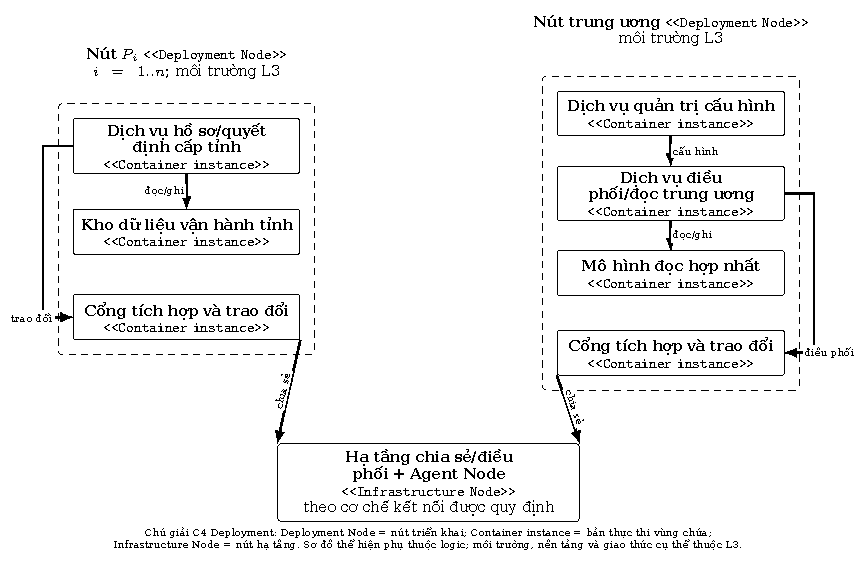
\includegraphics[width=0.96\textwidth]{figure_sources/fig05_c4_deployment_pdist.pdf}
\caption{Profile P-DIST -- góc nhìn triển khai dùng trong đánh giá.}
\end{figure}

\small
\renewcommand{\arraystretch}{1.02}
\setlength{\tabcolsep}{2pt}
\begin{center}
\begin{tabularx}{0.98\textwidth}{@{}p{2.0cm}p{3.0cm}X p{2.2cm}@{}}
\toprule
\textbf{Vùng/đối tượng} & \textbf{Quyền và dữ liệu} & \textbf{Kiểm soát kiến trúc bắt buộc} & \textbf{Chủ kiểm toán} \\
\midrule
Z1. Kênh người dùng & DN và cán bộ truy cập hồ sơ theo vai trò và phạm vi được cấp. & Xác thực qua nguồn phù hợp; ủy quyền theo vai trò/phạm vi; ghi mục đích và sự kiện truy cập đối với thao tác cần kiểm toán. & Đơn vị vận hành dịch vụ và cơ quan xử lý hồ sơ. \\
\addlinespace
Z2. Nút tỉnh & Quyền ghi đối với hồ sơ/quyết định thuộc thẩm quyền; dữ liệu nhạy cảm chỉ cho vai trò được phép. & Tách quyền theo địa bàn; cấu hình có phiên bản; nhật ký thay đổi trạng thái/quyết định; nhãn phân loại và hạn chế truy cập. & Cơ quan tỉnh và đơn vị vận hành nút tỉnh. \\
\addlinespace
Z3. Biên liên thông & Chỉ trao đổi trường dữ liệu nằm trong hợp đồng và mục đích được phép. & Kiểm tra nguồn/đích, lược đồ, phiên bản; bảo vệ kênh; chống xử lý trùng cho thông điệp nghiệp vụ; lưu bằng chứng gửi--nhận. & Đơn vị vận hành tích hợp; nhật ký phía gửi và nhận. \\
\addlinespace
Z4. Trung ương & Đọc/tổng hợp toàn quốc; phân phối mô hình nền và cấu hình; không sửa thay quyết định pháp lý của tỉnh. & Tách đặc quyền trung ương--tỉnh; lưu nguồn, độ mới và phiên bản; kiểm soát phát hành cấu hình; theo dõi thay đổi/đối soát. & Cơ quan trung ương và đơn vị vận hành nền tảng. \\
\addlinespace
Z5. Hệ thống nguồn ngoài & Nền tảng chỉ đọc/xác minh theo quyền được cấp, trừ khi hợp đồng nguồn quy định khác. & Không nhân bản quyền sở hữu dữ liệu; lưu định danh nguồn và thời điểm; áp dụng điều kiện truy cập và nhật ký của hệ thống nguồn. & Chủ quản hệ thống nguồn và đầu mối tích hợp. \\
\bottomrule
\end{tabularx}
\end{center}
\normalsize

Điều kiện an toàn thông tin đối với kết nối định danh điện tử và các nghĩa vụ bảo vệ dữ liệu được xem là điều kiện trước triển khai. Ma trận trên chỉ chỉ ra nơi kiến trúc phải đặt kiểm soát và bằng chứng; việc đạt cấp độ an toàn, thông lượng, tính sẵn sàng hoặc thời gian phục hồi chỉ có thể được xác nhận trên hệ thống hiện thực hóa.



\section*{S9. Chi tiết hình thức hóa kiến trúc}
Phần này lưu các chi tiết được chuyển khỏi thân bài để bài chính tập trung vào lập luận khoa học. Các mã AD/VP/CR tiếp tục được giữ nhằm cho phép đối chiếu với dữ liệu máy đọc được và kết quả đánh giá.

\subsection*{S9.1. Điểm biến thiên VP1--VP8}
\small
\renewcommand{\arraystretch}{1.02}
\setlength{\tabcolsep}{2.2pt}
\begin{longtable}{@{}p{0.75cm}p{3.6cm}p{5.1cm}p{5.5cm}@{}}
\toprule
\textbf{Mã} & \textbf{Điểm biến thiên} & \textbf{Lõi không được phá vỡ} & \textbf{Các lựa chọn điển hình} \\
\midrule
\endfirsthead
\toprule
\textbf{Mã} & \textbf{Điểm biến thiên} & \textbf{Lõi không được phá vỡ} & \textbf{Các lựa chọn điển hình} \\
\midrule
\endhead
\bottomrule
\endfoot
VP1 & Chiến lược hợp nhất dữ liệu tỉnh--trung ương & Quyền ghi được gán theo thời gian với một writer hợp lệ; mô hình đọc trung ương không thay thế nguồn pháp lý địa phương. & Truy vấn theo yêu cầu; đồng bộ một phần; đồng bộ toàn bộ miền được phép; kết hợp theo tập dữ liệu. \\
VP2 & Công nghệ luồng/quy tắc và cấu hình địa phương & Mô hình nền pháp lý và cổng kiểm tra không đổi; cấu hình/lược đồ có phiên bản, cửa sổ tương thích và quy tắc cho hồ sơ đang chạy. & Workflow/rule engine; máy trạng thái dịch vụ; BPMN/mô hình cấu hình; kết hợp. \\
VP3 & Mẫu tương tác theo giao diện & Thay đổi trạng thái có định danh, dấu thời gian, tính lũy đẳng và nhật ký. & API đồng bộ; sự kiện/thông điệp; kết hợp. \\
VP4 & Biên với hệ thống TTHC/dịch vụ công & Không thay thế vai trò kênh có thẩm quyền; hợp đồng dữ liệu rõ. & Tích hợp nhúng; API; sự kiện; tham chiếu thủ công dự phòng. \\
VP5 & Mô hình phân quyền nội bộ & Đặc quyền tối thiểu, phạm vi thẩm quyền, mục đích và nhật ký. & RBAC; ABAC; kết hợp. \\
VP6 & Lưu quan hệ hệ sinh thái & Quan hệ không bị cắt bởi địa giới; có nguồn và thời gian hiệu lực. & Quan hệ; đồ thị; kết hợp. \\
VP7 & Topology lưu trữ và cấu trúc triển khai & Giữ biên quyền ghi theo thẩm quyền; biên tích hợp và biên tin cậy được mô tả bất kể topology. & Kho tập trung đa tenant; phân vùng logic/schema; P-DIST; mô hình lai. \\
VP8 & Bộ thích nghi, giao thức và lược đồ nguồn ngoài & Giữ thẩm quyền nguồn, ngữ nghĩa, provenance và phiên bản. & API; thông điệp; tệp/lô; truy vấn; lược đồ theo nguồn. \\
\end{longtable}
\normalsize

\subsection*{S9.2. Chi tiết hai quyết định được tinh chỉnh sau stress-test}
\textbf{AD01 -- biên quyền ghi theo thẩm quyền.} B1-R biểu diễn gán quyền ghi theo \texttt{write\_scope} (subject/aggregate hoặc \texttt{case\_id}) cùng \texttt{jurisdiction\_id}, khoảng hiệu lực, \texttt{source\_evidence}, \texttt{transfer\_id} và \texttt{writer\_epoch} tăng đơn điệu; mutation dùng epoch cũ bị từ chối. Chuyển giao theo chuỗi \textsc{prepared--old-frozen--cutover-confirmed--new-active--completed}; chỉ hủy trước \textsc{new-active}, sau đó phục hồi tiến về trước. Hồ sơ đang chạy được gán đúng một writer theo kế hoạch chuyển. Topology vẫn là VP7; cấu hình dùng trong stress-test là P-DIST. Chi tiết này là ngữ nghĩa thiết kế L2, không khóa thuật toán consensus, cơ chế khóa hay middleware L3.

\textbf{AD03 -- mô hình nền pháp lý và cấu hình địa phương.} B1-R giữ trạng thái, cổng quyết định và thời hạn L1 trong mô hình nền; địa phương chỉ cấu hình bước nội bộ, vai trò, biểu mẫu và mục tiêu xử lý. Mỗi cấu hình có phiên bản/ngày hiệu lực và qua cổng kiểm tra. Sau S10, hợp đồng/lược đồ/cấu hình còn phải công bố cửa sổ tương thích và phiên bản tối thiểu còn hỗ trợ; hồ sơ đang xử lý được ghim vào phiên bản quy trình cho đến khi có quy tắc chuyển minh thị.

Bản ghi đầy đủ của AD01--AD05, bao gồm issue, alternatives, rationale, trade-offs, constraints, elements và variation points, nằm trong \texttt{architecture\_decisions.csv}.

\subsection*{S9.3. Quy tắc phù hợp của lõi và profile P-DIST}
\small
\renewcommand{\arraystretch}{1.02}
\setlength{\tabcolsep}{2.4pt}
\begin{longtable}{@{}p{0.9cm}p{9.5cm}p{4.2cm}@{}}
\toprule
\textbf{Mã} & \textbf{Quy tắc} & \textbf{Bằng chứng kiến trúc tối thiểu} \\
\midrule
\endfirsthead
\toprule
\textbf{Mã} & \textbf{Quy tắc} & \textbf{Bằng chứng kiến trúc tối thiểu} \\
\midrule
\endhead
\bottomrule
\endfoot
CR1 & Mọi hành vi thực hiện nghĩa vụ pháp lý phải truy được tới Cxx.yy lớp A và AD/AE liên quan. & Ma trận truy vết và hồ sơ quyết định. \\
CR2 & Mọi thao tác thay đổi trạng thái phải kiểm tra gán quyền ghi đang hiệu lực đối với phạm vi ghi được khai báo. & Policy/sequence kiểm tra quyền và audit. \\
CR3 & Tại một thời điểm chỉ một writer hợp lệ đối với cùng \texttt{write\_scope}; ghi từ gán cũ phải bị từ chối. & Bất biến single-active-writer và \texttt{writer\_epoch}. \\
CR4 & Thẩm quyền dữ liệu được gán theo nhóm thuộc tính và phân biệt legal authority, create/update authority, SoR và distribution source. & Ma trận thẩm quyền dữ liệu. \\
CR5 & Cấu hình địa phương không được nới thẩm quyền, trạng thái quyết định hoặc thời hạn L1 và phải qua cổng kiểm tra trước kích hoạt. & Baseline pháp lý và conformance gate. \\
CR6 & Hợp đồng, lược đồ và quy trình phải có phiên bản, ngày hiệu lực, cửa sổ tương thích và quy tắc xử lý hồ sơ đang chạy. & Registry phiên bản và compatibility policy. \\
CR7 & Mô hình đọc AE25 phải công bố nguồn, độ mới, phiên bản và không được dùng như nguồn ban hành quyết định pháp lý. & Metadata/provenance và nhãn nguồn. \\
CR8 & Luồng chia sẻ bắt buộc phải giữ định danh, tính lũy đẳng, bằng chứng gửi--nhận và thử lại có kiểm soát. & Exchange log, receipt, retry policy. \\
CR9 & Quan hệ hệ sinh thái xuyên địa bàn phải giữ định danh chủ thể, nguồn, khoảng hiệu lực và không bị nhân bản theo biên thẩm quyền. & Relationship model và lineage. \\
PD1 & Trong profile P-DIST, mỗi nút nghiệp vụ tỉnh được ánh xạ tới một kho vận hành vật lý tách biệt và lớp trung ương chỉ giữ mô hình đọc/điều phối. & V5 deployment profile. \\
PD2 & Profile P-DIST phải mô tả biên lỗi, phục hồi, độ mới và giao thức chuyển quyền giữa các kho vật lý. & V5/V6 và kiểm thử hậu triển khai. \\
\end{longtable}
\normalsize

\subsection*{S9.4. Ánh xạ nhóm năng lực tới đáp ứng kiến trúc}
Bảng này lưu mức chi tiết đã được rút khỏi thân bài. Các locator Cxx.yy đầy đủ vẫn nằm trong ma trận truy vết nguyên tử.

\small
\renewcommand{\arraystretch}{1.02}
\setlength{\tabcolsep}{2.4pt}
\begin{longtable}{@{}p{3.0cm}p{5.0cm}p{6.5cm}@{}}
\toprule
\textbf{Nhóm năng lực} & \textbf{Nguồn/vị trí đại diện} & \textbf{Đáp ứng kiến trúc} \\
\midrule
\endfirsthead
\toprule
\textbf{Nhóm năng lực} & \textbf{Nguồn/vị trí đại diện} & \textbf{Đáp ứng kiến trúc} \\
\midrule
\endhead
\bottomrule
\endfoot
Định danh pháp lý DN & C04.02, C05.08--C05.10, C06.12; Luật Dữ liệu; NĐ 278; QĐ 1973 & Tham chiếu/đồng bộ nguồn quốc gia; không tạo lại dữ liệu chủ; định danh được tách khỏi trạng thái chuyên ngành. \\
Công nhận DN KNST & C03.02--C03.30; các Điều 35, 39, 41, 43--45 NĐ 268 & Quản lý hồ sơ tiêu chí, hội đồng, trạng thái, hiệu lực giấy, cấp lại/chấm dứt và lịch sử quyết định. \\
Chứng nhận DN KH\&CN & C03.31--C03.43; các Điều 48, 50--53 NĐ 268 & Tiếp nhận, thẩm định, cấp lại, hậu kiểm; khóa các cổng pháp lý nhưng cho phép biến thiên bước nội bộ. \\
Thông báo/báo cáo liên cấp & C03.44, C03.46, C03.48; Điều 54 và Điều 66 NĐ 268 & Nút tỉnh tạo bản ghi nguồn; lớp trung ương nhận bản đọc/thông báo, giám sát hạn và tổng hợp. \\
Dữ liệu chủ, danh mục, siêu dữ liệu & C02/C04/C05/C06 liên quan; QĐ 2439, NĐ 278, QĐ 1973 & Từ điển/danh mục dùng chung, ánh xạ mã, nguồn, chất lượng, phiên bản và lịch sử thay đổi. \\
Nút dữ liệu tỉnh và mô hình đọc trung ương & C03.31--C03.48, C05.13--C05.16 & Phân vùng quyền ghi theo thẩm quyền; đồng bộ/truy vấn có provenance và độ mới; topology là điểm biến thiên. \\
Cấu hình quy trình & C03.10--C03.14, C03.27--C03.30, C03.40--C03.42 & Mô hình nền L1 kết hợp cấu hình địa phương có phiên bản và cổng kiểm tra tuân thủ. \\
Liên thông dữ liệu & C05.02, C05.13--C05.16, C06.09--C06.10 & Tích hợp qua hạ tầng chia sẻ/điều phối được quy định; không tạo trục điểm--điểm song song cho luồng bắt buộc. \\
Định danh/xác thực & C08.01, C08.06--C08.09; NĐ 69 & Sử dụng nguồn định danh/xác thực có thẩm quyền; quyền nghiệp vụ vẫn thuộc miền quản lý. \\
An toàn và dữ liệu cá nhân & C09.01--C09.05; Luật 91; NĐ 356 & Phân loại, biên tin cậy, phân quyền, nhật ký và vòng đời dữ liệu; mức đạt thực tế phải kiểm chứng sau triển khai. \\
Năng lực mở rộng & Không có ràng buộc A trực tiếp & Các chức năng mở rộng chỉ ở L3 sau khi yêu cầu và tiêu chí đánh giá được xác nhận. \\
\end{longtable}
\normalsize

\section*{S10. Chi tiết mô hình thẩm quyền dữ liệu}
Phần này lưu các chi tiết được rút khỏi Mục kiến trúc dữ liệu của thân bài. Chúng phục vụ kiểm tra cách hiện thực hóa các bất biến về thẩm quyền, nguồn gốc và chuyển giao quyền ghi; các tên trường chỉ là biểu diễn tham chiếu ở mức L2, không phải schema bắt buộc của một sản phẩm phần mềm.

\subsection*{S10.1. Bản ghi gán quyền ghi và chuyển giao}
Một bản ghi gán quyền ghi có thể mang bốn nhóm trường tham chiếu:
\begin{itemize}
\item chủ thể và phạm vi: \texttt{subject\_id}, \texttt{write\_scope} hoặc \texttt{case\_id};
\item địa bàn và hiệu lực: \texttt{jurisdiction\_id}, \texttt{valid\_from}, \texttt{valid\_to};
\item bằng chứng và giao dịch chuyển quyền: \texttt{source\_evidence}, \texttt{transfer\_id};
\item phiên writer: \texttt{writer\_epoch}.
\end{itemize}
Bất biến cần bảo toàn là: tại một thời điểm, mỗi phạm vi chỉ có tối đa một writer đang hiệu lực; mọi mutation phải mang epoch hiện hành và ghi bằng epoch cũ bị từ chối.

Chuỗi trạng thái tham chiếu cho chuyển giao là
\[
\textsc{prepared}\rightarrow\textsc{old-frozen}\rightarrow\textsc{cutover-confirmed}\rightarrow\textsc{new-active}\rightarrow\textsc{completed}.
\]
Trước \textsc{new-active}, chuyển giao có thể bị hủy; sau khi epoch mới đã được kích hoạt, phục hồi phải tiến về trước thay vì quay lại epoch cũ. Hồ sơ đang xử lý phải được đưa vào kế hoạch chuyển với đúng một writer hợp lệ. Writer mới chỉ được kích hoạt sau khi có bằng chứng đóng băng writer cũ và hoàn thành đối soát dữ liệu/nguồn gốc. Khi một nút khởi động lại sau gián đoạn, nó phải xác minh epoch hiện hành trước khi cho phép ghi. Cơ chế khóa, consensus hoặc middleware cụ thể thuộc L3.

\subsection*{S10.2. Ma trận nguồn/thẩm quyền chi tiết}
\small
\setlength{\tabcolsep}{2.4pt}
\renewcommand{\arraystretch}{1.02}
\begin{longtable}{@{}p{3.0cm}p{5.2cm}p{6.2cm}@{}}
\toprule
\textbf{Nhóm dữ liệu} & \textbf{Nguồn/vai trò có thẩm quyền} & \textbf{Vai trò của nền tảng} \\
\midrule
\endfirsthead
\toprule
\textbf{Nhóm dữ liệu} & \textbf{Nguồn/vai trò có thẩm quyền} & \textbf{Vai trò của nền tảng} \\
\midrule
\endhead
\bottomrule
\endfoot
Định danh pháp lý DN & CSDL quốc gia về doanh nghiệp là nguồn tham chiếu/định danh theo Luật Dữ liệu, NĐ 278 và QĐ 1973. & Tham chiếu hoặc đồng bộ khóa và thuộc tính cần thiết; không tạo lại tên, mã hay trạng thái đăng ký như một bản chủ song song. \\
\addlinespace
Trạng thái/giấy DN KH\&CN & Cơ quan tỉnh có thẩm quyền tạo quyết định theo NĐ 268; nút đang có gán quyền ghi hiệu lực là SoR nghiệp vụ cho trạng thái chuyên ngành thuộc phạm vi đó. & Trung ương nhận bản đọc/thông báo để giám sát, tổng hợp và định tuyến; luôn giữ nguồn, phiên bản và thời điểm đồng bộ. \\
\addlinespace
Trạng thái/giấy DN KNST & Cơ quan tỉnh có thẩm quyền tạo quyết định theo NĐ 268; nút đang có gán quyền ghi hiệu lực là SoR nghiệp vụ cho phạm vi đó. & Quản lý vòng đời tại tỉnh; trung ương lưu bản đọc/tổng hợp, bằng chứng trao đổi và thông tin định tuyến quyền ghi. \\
\addlinespace
Minh chứng, năng lực và báo cáo & Nguồn cụ thể phụ thuộc từng loại kết quả, văn bằng hoặc báo cáo; QĐ 1973 và dự thảo khung tiêu chí cung cấp mô tả miền dữ liệu. & Lưu tham chiếu hoặc dữ liệu nghiệp vụ cần thiết kèm trạng thái xác minh; dữ liệu tự khai không tự trở thành dữ liệu chủ đã xác thực. \\
\addlinespace
Quan hệ hệ sinh thái & Quan hệ có thể vượt địa giới; thẩm quyền của từng thuộc tính đầu mối vẫn theo nguồn của chủ thể tương ứng. & Lưu liên kết có nguồn, thời gian hiệu lực và địa bàn hai đầu; không nhân bản cùng một quan hệ thành nhiều ``sự thật'' theo tỉnh. \\
\addlinespace
Danh mục/từ điển & Kế thừa khung, từ điển và danh mục cấp trên theo NĐ 278 và QĐ 1973. & Mở rộng chuyên ngành có phiên bản và ánh xạ, không phá mã dùng chung. \\
\addlinespace
Siêu dữ liệu/nguồn gốc & Luật Dữ liệu, NĐ 278 và QĐ 1973 yêu cầu mô tả nguồn, chất lượng, phiên bản và khả năng liên thông. & Gắn nguồn, thời điểm, trạng thái xác minh, phiên bản và lịch sử thay đổi để hỗ trợ kiểm toán/đối soát. \\
\addlinespace
Dữ liệu tổng hợp/mở & Là dữ liệu dẫn xuất từ các nguồn có thẩm quyền, không phải nguồn pháp lý mới. & Mọi tập dẫn xuất phải truy nguyên về tập nguồn/phiên bản và không thay thế nguồn đầu vào. \\
\end{longtable}
\normalsize

\subsection*{S10.3. Chuẩn hóa và các điểm chẩn đoán từ nguồn dự thảo}
Dự thảo khung tiêu chí đề xuất hệ mã DC/MD/F/LC/SYS, mã quốc gia/ngôn ngữ, UTF-8, các định dạng trao đổi và siêu dữ liệu nguồn--thời gian--trạng thái--phiên bản. Do đây là nguồn lớp D, các quy ước chỉ được dùng để kiểm tra khả năng tương thích, không tạo nghĩa vụ L1.

Ba điểm chẩn đoán được giữ để theo dõi khi văn bản chính thức thay đổi: (i) dự thảo còn viện dẫn NĐ 47/2020/NĐ-CP trong khi NĐ 278 đã làm văn bản này hết hiệu lực; (ii) MD001 cần được phân tách ở mức thuộc tính giữa định danh pháp lý và trạng thái chuyên ngành để không tạo một ``bản ghi gốc'' cạnh tranh với nguồn quốc gia; và (iii) phạm vi CSDL được liệt kê trong QĐ 1762 chưa hoàn toàn trùng với hai miền DN KH\&CN và DN KNST của dự thảo. Các điểm (ii)--(iii) chỉ mang trạng thái \textsc{cần làm rõ}; chúng không được nâng thành xung đột hoặc dùng để khóa topology khi chưa có quyết định có thẩm quyền.



\section*{S11. Mười họ ràng buộc kiến trúc và hệ quả thiết kế}
Phần thân bài chỉ sử dụng bốn sức ép kiến trúc tổng hợp. Bảng này bảo toàn phân nhóm C01--C10 và các locator đại diện để có thể đối chiếu với \texttt{constraint\_traceability.}\allowbreak\texttt{csv}. Con số trong ngoặc là số dòng truy vết thuộc họ; A/D/M là lớp nguồn.

\small
\renewcommand{\arraystretch}{1.02}
\setlength{\tabcolsep}{2.3pt}
\begin{longtable}{@{}p{1.15cm}p{4.0cm}p{4.9cm}p{4.35cm}@{}}
\toprule
\textbf{Mã} & \textbf{Nguồn/vị trí đại diện} & \textbf{Ràng buộc rút gọn} & \textbf{Hệ quả kiến trúc} \\
\midrule
\endfirsthead
\toprule
\textbf{Mã} & \textbf{Nguồn/vị trí đại diện} & \textbf{Ràng buộc rút gọn} & \textbf{Hệ quả kiến trúc} \\
\midrule
\endhead
\bottomrule
\endfoot
C01 (6; A) & QĐ 3090, Điều 1; QĐ 292, Chương 2 Mục II & Đặt hệ thống chuyên ngành trong các mô hình tham chiếu quốc gia/chính phủ số. & Mô tả đa góc nhìn; truy vết mỗi miền kiến trúc về khung tương ứng. \\
\addlinespace
C02 (4; A) & QĐ 2439, Điều 1; Khung kèm theo Chương I Mục I.1 & Thống nhất kiến trúc, quản trị và từ điển dữ liệu. & Kế thừa từ điển, mã, siêu dữ liệu và quản trị vòng đời. \\
\addlinespace
C03 (48; A) & Luật 93, khoản 3 Điều 20; NĐ 268: các Điều 35, 39, 43, 48, 51--54, 66 & Hai chuỗi nghiệp vụ có thẩm quyền tỉnh, vòng đời giấy, hội đồng, thời hạn và nghĩa vụ liên cấp. & Máy trạng thái, thời hạn, lịch sử quyết định, cấu hình quy trình và đồng bộ tỉnh--trung ương. \\
\addlinespace
C04 (8; A) & Luật Dữ liệu: Điều 11--13 & Không thu thập lại dữ liệu đã chia sẻ; quản lý chất lượng và phân loại. & Tham chiếu nguồn chính thức; lưu nguồn gốc, chất lượng, phân loại và kiểm soát truy cập. \\
\addlinespace
C05 (18; A) & NĐ 278: Điều 4--7, 23--24 & Chia sẻ qua hạ tầng quy định; một nguồn tin cậy; truy vấn/đồng bộ; yêu cầu chuyển tiếp. & Liên thông trung gian, xác lập nguồn theo thuộc tính, nhật ký và quản trị đồng bộ. \\
\addlinespace
C06 (14; A) & QĐ 1973, Mục II.1--II.2; III.1.4; III.3.2--III.3.3; Phụ lục Mục 3 & Tránh trùng lặp, xác định điểm tạo lập; doanh nghiệp lấy từ nguồn quốc gia; dữ liệu chuyên ngành quản trị ở cấp Bộ. & Tách định danh pháp lý khỏi trạng thái chuyên ngành; tích hợp qua hạ tầng chia sẻ theo khung của Bộ. \\
\addlinespace
C07 (9; A+D) & QĐ 1762, Phụ lục STT 38; dự thảo Điều 4 và Phụ lục IV/IX & Danh mục hiện hành và dự thảo chưa hoàn toàn trùng phạm vi; dự thảo yêu cầu một nguồn chính thức. & Giữ trạng thái cần làm rõ về phạm vi CSDL; dùng dự thảo để chẩn đoán, không tạo L1. \\
\addlinespace
C08 (9; A) & NĐ 69: Điều 12, 18--19; NĐ 169, Điều 43 & Dùng định danh/xác thực có thẩm quyền và đáp ứng điều kiện kết nối. & Tách xác thực danh tính khỏi phân quyền nghiệp vụ nội bộ. \\
\addlinespace
C09 (6; A) & Luật 91: Điều 19, 37; NĐ 356, Điều 4 & Bảo vệ dữ liệu cá nhân, giới hạn truy cập và duy trì biện pháp quản lý/kỹ thuật. & Phân loại, phân quyền, nhật ký, vòng đời và biên tin cậy. \\
\addlinespace
C10 (6; M) & EIF, Hình 3 tr.22, tr.27--30; EU 2024/903, Điều 3 và 6 & Kiểm tra liên thông theo bốn lớp EIF. & Ma trận liên thông; nguồn EU chỉ là tham chiếu phương pháp. \\
\end{longtable}
\normalsize


\section*{S12. Ma trận đánh giá kịch bản chi tiết}
Phần này giữ các neo kiến trúc và phép kiểm tra chi tiết đã được rút khỏi thân bài. Bảng chính chỉ trình bày phát hiện có ý nghĩa đối với lập luận khoa học; các nội dung dưới đây phục vụ truy vết và chuẩn bị kiểm chứng nguyên mẫu.

\small
\setlength{\tabcolsep}{2.1pt}
\renewcommand{\arraystretch}{1.02}
\begin{longtable}{@{}p{3.1cm}p{1.7cm}p{1.7cm}p{3.1cm}p{5.0cm}@{}}
\toprule
\textbf{Kịch bản} & \textbf{B1$_0$} & \textbf{B1-R} & \textbf{Neo kiến trúc} & \textbf{Kiểm chứng hiện thực hóa cần thiết} \\
\midrule
\endfirsthead
\toprule
\textbf{Kịch bản} & \textbf{B1$_0$} & \textbf{B1-R} & \textbf{Neo kiến trúc} & \textbf{Kiểm chứng hiện thực hóa cần thiết} \\
\midrule
\endhead
\bottomrule
\endfoot
S1. Tỉnh xử lý/quyết định theo thẩm quyền & Trực tiếp & Trực tiếp & AD01, AE24, CR2 & Định tuyến theo phạm vi và từ chối ghi ngoài phạm vi đang có hiệu lực. \\
S2. Hai tỉnh khác bước nội bộ & Trực tiếp & Trực tiếp & AD03, AE26, CR5 & Kiểm tra cấu hình địa phương không nới trạng thái, thẩm quyền hay thời hạn L1. \\
S3. Quy định thay đổi & Có điều kiện & Có điều kiện & AD03, CR6 & Hồi quy cấu hình; phát hành phiên bản mới; xử lý hồ sơ đang chạy và lịch sử. \\
S4. Chia sẻ trung ương gián đoạn & Có điều kiện & Có điều kiện & AD04, CR8 & Gửi lại có kiểm soát, chống xử lý trùng, bảo toàn trạng thái và thời hạn nghiệp vụ. \\
S5. Ảnh dữ liệu toàn quốc & Có điều kiện & Có điều kiện & AE25, CR7 & Đo độ mới, kiểm tra provenance/phiên bản và đối soát với nguồn tạo lập. \\
S6. Định danh doanh nghiệp đổi ở nguồn quốc gia & Có điều kiện & Có điều kiện & AE03, AE15, CR4 & Làm mới/xác minh nguồn và xử lý thay đổi khóa/tham chiếu mà không tạo bản chủ cạnh tranh. \\
S7. Lớp trung ương không sẵn sàng & Có điều kiện & Có điều kiện & AD04, V4/V5 & Thử miền lỗi và xác minh bước nào được tiếp tục, dừng hoặc khôi phục theo phụ thuộc ngoài. \\
S8. Quan hệ xuyên tỉnh & Có điều kiện & Có điều kiện & AD05, CR9 & Hợp nhất quan hệ theo định danh, nguồn, hai đầu quan hệ và thời gian hiệu lực. \\
S9. Chuyển phạm vi quản lý A--B & Rủi ro & Có điều kiện & AD01, CR2--CR3 & Ghi cạnh tranh, cutover, khởi động lại, gửi lại và forward recovery phải giữ single-active-writer/provenance. \\
S10. Nâng lược đồ/quy trình lệch thời điểm & Có điều kiện & Có điều kiện & AD03, CR6 & Ma trận tương thích, nâng cấp cuốn chiếu, version pinning và phát lại dữ liệu lịch sử. \\
\end{longtable}
\normalsize

Chi tiết L2 của chuyển quyền ghi theo thời gian được mô tả ở S9.2 và S10.1; chi tiết quản trị tương thích phiên bản nằm ở S9.2. Các phép kiểm tra trên chưa được thực hiện trong nghiên cứu hiện tại và không được diễn giải như kết quả prototype.

\end{document}
